Purpose of chapter, TODO

\section{Python performance and parallel capabilities}
There are several implementations of the Python language. This section will focus on CPython, the canonical and most popular
Python implementation \cite{pythonimplementations_ppw}, and also the one that TriOptima uses. This thesis uses Python 2.7.

\subsection{Performance}
The general performance of CPython is slower than other popular languages such as C and Java for several
reasons \cite{barany_2014_python_pipd}. Overhead is introduced due to the fact that all operations need to dispatched dynamically,
and accessing data demands the dereferencing of a pointer to a heap data structure. Also, the fact that late binding is employed
for function calls, the automatic memory memory management in the form of reference counting, and the boxing and unboxing of
methods contribute to the at times poor performance.

\subsection{The GIL, Global Interpreter Lock}
In order to simplify the implementation and to avoid concurrency related bugs in the CPython interpreter,
a mechanism called the Global Interpreter Lock - or the GIL - is employed  \cite{palach_2014_parallel_ppwp}.
The GIL locks the entire CPython interpreter, making it impossible for multiple Python threads to make progress at
the same time, thereby removing the benefits of parallel CPU bound calculations
\cite{glossary_gp2d}. When an I/O operation is started from Python, the GIL is released.
Efforts to remove the GIL have been made, but have as of yet been unsuccessful.

\subsection{Threading}
The Python \code{threading} module provides a multitude of utilities for concurrent programming, such as an object abstraction of
threads, locks, semaphores, and condition objects \cite{16_1thtip2d}. When using the \code{threading} module in CPython, the GIL is in
effect, disallowing true parallelism and hampering efficient use of multicore machines. When performing I/O bound operations, the
\code{threading} module can be used to improve performance; at times significantly \cite[p. 121-124]{slatkin_2015_effective_ep5swtwbp}

\subsection{Multiprocessing}
The \code{multiprocessing} module has a similar API to the \code{threading} module, but avoids the negative effects of the GIL by spawning
separate processes instead of user threads. This works since the processes have separate GILs, which do not affect each other and
enables the processes to utilize true parallelism \cite{slatkin_2015_effective_ep5swtwbp}. The processes are represented by the \code{multiprocessing.Process} class.

The \code{multiprocessing} module provides mechanisms for performing IPC.
In order for the data to be transferred between processes, it needs to be serializable through the use of the Python \code{pickle}
module \cite[p. 143]{slatkin_2015_effective_ep5swtwbp}. When transferring data, it is serialized, sent to another process through
a local socket, and then deserialized. These operations, in conjunction with the creation of the processes, gives the
\code{multiprocessing} module a high overhead when communicating between processes.

The two main facilities that the \code{multiprocessing} module provides for IPC are \cite{palach_2014_parallel_ppwp}:
\begin{itemize}
  \item \code{multiprocessing.Pipe}, which serves as a way for two processes to communicate using the operations \code{send()}
    and \code{recv()} (receive). The pipe is represented by two connection objects which correspond to each end of the pipe.
    See figure \ref{fig:code_pipe_example} for an example.
  \item \code{multiprocessing.Queue}, which closely mimics the behaviour and API of the standard Python \code{queue.Queue}, but
    can be used by several processes at the same time without concurrency issues. This \code{multiprocessing} queue internally
    synchronizes access by multiple processes using locks, and uses a \emph{feeder thread} to transfer data to other processes.
    See figure \ref{fig:code_queue_example} for an example.
\end{itemize}

In addition to the parallel programming utilities mentioned above, the \code{multiprocessing} module provides the \code{Pool} abstraction
for specifying a number of workers as well as several ways of assigning functions for the workers to be performed in parallel. For
example, a programmer can use \code{Pool.map} to make the workers in the pool execute a specified function on each element in a
collection.
See figure \ref{fig:code_pool_example} for an example.

\begin{figure}[ht]
  \centering
  \pythonexternal{code_examples/pipe_example.py}
  \caption{\code{multiprocessing.Pipe} example}
  \label{fig:code_pipe_example}
\end{figure}

\begin{figure}[ht]
  \centering
  \pythonexternal{code_examples/queue_example.py}
  \caption{\code{multiprocessing.Queue} example}
  \label{fig:code_queue_example}
\end{figure}

\begin{figure}[ht]
  \centering
  \pythonexternal{code_examples/pool_example.py}
  \caption{\code{multiprocessing.Pool} example}
  \label{fig:code_pool_example}
\end{figure}


\section{Technology}
In this section, technologies used in triResolve that will be mentioned throughout this chapter are briefly described.

\subsection{Django}
Django is a Python web development framework \cite{holovaty_chapter_c1itd}. It implements a version of the MVC (Model-View-Controller) pattern, which decouples request routing, data access, and
presentation. Django's model layer allows the programmer to retrieve and modify entities in an SQL database through Python code, without writing SQL.

\subsection{MySQL}
MySQL is an open source relational database system \cite{what_wim}. It is used by TriOptima as the database backend for Django.

\subsection{Cassandra}
Cassandra is a column-oriented \textit{NoSQL} database \cite[p. 1-9]{mishra_2014_beginning_bacd}. It features dynamic schemas, meaning that columns can be added dynamically to a schema as needed, and that
the number of columns may vary from row to row. Cassandra is designed to have no single point of failure, and uses a number of nodes in a peer-to-peer structure. This design is
employed in order to ensure high availability, with data replicated across the nodes.

\section{Performance analysis tools}
\subsection{cProfile}
A Python profiler with a relatively low overhead, which can be invoked both directly in a Python program and form the command line \cite{26_2tppp2d}.

\subsection{resource}
\code{resource} is a Python module used for measuring resources used by a Python program \cite{36_3rruip2d}. It can be used for finding the user time, system time,
and the maximum memory used by the process.

\section{Hardware}
\begin{itemize}
  \item Laptop computer with several cores (supplied by TriOptima), for working and initial small-scale testing and profiling. This is a MacBook Pro running OSX, with an Intel Core i7 processor and 4 physical cores.
    The processor supports hyperthreading, bringing the number of logical cores to 8.
  \item For the main evaluation, TriOptima’s acceptance test environment, with hardware similar to what is used in production, was used. This is a stationary computer running Linux CentOS, with a dual processor
    architecture. The processors are 2 Intel Xeon E5504 processors with 4 cores each, making a total of 8 cores. The cores do not support hyperthreading.
\end{itemize}

\section{Trade files and datasets}
As mentioned briefly in section \ref{trioptima}, users of the triResolve service upload \textit{trade files}, which contain one or several datasets with
rows of trade data such as party id, counterparty id, trade id, notional, and so on. An example of a trade dataset (with some columns omitted) can be seen in figure
\ref{fig:data_set_example}.

\begin{figure}[ht]
\centering
\resizebox{\linewidth}{!}{%
\begin{tabular}{|c|c|c|p{3cm}|c|c|}%
  \hline
  \bfseries Party ID & \bfseries CP ID & \bfseries Trade ID & \bfseries Product class & \bfseries Trade curr & \bfseries Notional
  \csvreader[respect all,head to column names]{figures/EFET.csv}{PARTY_ID=\pid, CP_ID=\cpid, TRADE_ID=\tid, PRODUCT_CLASS=\pcls, TRADE_CURR=\tc, NOTIONAL=\notional}
  {\\\hline \pid & \cpid & \tid & \pcls & \tc & \notional}
  \\ \hline
\end{tabular}}
  %\centering
\caption[Example of trade dataset]{A simplified example of a trade dataset uploaded by the users of triResolve.}
  \label{fig:data_set_example}
\end{figure}

\section{File formats}
Different customers may have different ways of formatting their datasets, with different names for headers, varying column orders, extra fields,
and special rules. In order to convert these into a standard format that make it possible to use the files in the same contexts, a file format specifying
how the dataset in question should be processed is used. The format contains a set of \textit{filters} which should be applied to each row of the dataset.
The different filter configurations may affect how parallelizable the processing of the dataset is.

\section{Verification results}
The result of the dataset processing is called a \textit{verification result}, and consists of one row per trade, with correctly modified values, in a Cassandra schema.
In addition, a row in the MySQL database consisting of metadata relating to the result as a whole is created. This metadata includes result owner, number of rows, time metrics, and so on.

\textit{Note: The verification results are not to be confused with the results of this thesis. They are part of the problem this thesis aims to solve.}

\section{Transformation with constraints}

\subsection{Filters}
All filters used to transform a dataset into a verification result are outlined below.

\begin{itemize}
\item \textbf{Header detection} --
There may be a number of initial lines in the dataset which do not contain the header (which specifies the column names). The header detection filter checks if a row is the header,
and if it is it saves the column names and corresponding indices for use in subsequent rows. If the row is not the header or the header has already been detected
(for example if another header row is encountered in the middle of the dataset), this filter terminates without any effect and the rest of the filters are applied.
This filter is included in all file formats.

\item \textbf{Mapping} --
Maps a value from a column in the dataset to a specified output column in the verification result. There is usually a mapping for each of the columns in the input
dataset, and the Mapping filter is therefore one of the most common filters. The mappings may have small extra tuning attached to them, such as specifying a date
format or extracting only part of the text using regex. One of these extra tunings is attached to the trade id column, and is called \textit{Make unique}.
This tuning keeps track of all trade id:s that have been encountered so far, and, if it finds a duplicate, adds a suffix to it in order to ensure that all trade id:s are unique.

\item \textbf{Dataset translation} --
A dataset translation is similar to a mapping, but uses specified columns in an external dataset to map input columns to output columns.

\item \textbf{Dataset information} --
Extracts information about the dataset, such as the name or owner.

\item \textbf{Tradefile information} --
Similar to the dataset information filter, except that it extracts information about the trade file that contains the dataset.

\item \textbf{Null translation} --
In some datasets, other values than \code{NULL} are used to convey the absence of a value. This filter allows the user to specify which other values
should be interpreted as \code{NULL}.

\item \textbf{Relation currency} --
If the currency that is supposed to be used in a relation (a party and a counterparty) is stored in the database and should be mapped to an output column, this
filter retrieves this information.

\item \textbf{Global variable} --
A global variable filter writes a value to a variable that is accessible by subsequent filters on the same row, and by all filters on the rest of the rows in the data
set. A global variable can be written several times throughout the processing of a dataset.

\item \textbf{State variable} --
A state variable is similar to a global variable, but is always written to before all other processing of the dataset begins.

\item \textbf{Temporary variable} --
Similar to the other variables, except for the fact that it is only accessible during processing of the row where it was written. When the 
processing of the row is finished, the variable is cleared.

\item \textbf{Conditional block} --
A conditional block works like the programming construct \code{if}. It performs a specified filter (which may also be a conditional block) only if a certain
condition is fulfilled. Most commonly, the condition takes the form '\code{field = value}', but may also involve more complex expressions in the form of a
subset of Python.

\item \textbf{Logger} --
A logger filter simply logs a given value. Can for instance be used when a user wants to know whenever a conditional block has been entered.

\item \textbf{Skip row} --
Ignores the current row when processing. Usually used in a conditional block.

\item \textbf{Stop processing} --
Stops processing the dataset, ignoring all subsequent rows. Can be used as a subfilter in the Conditional block filter when the footer of the dataset
contains information that should not be interpreted as a trade.

\item \textbf{Third party automapper} --
When a customer has uploaded a trade file on behalf of another customer, this filter extracts the information needed to make sure that the data is loaded
for the correct customer.

\item \textbf{Set value} --
Simply sets the value of the output column to the value that is entered.

\item \textbf{RegExp extract} --
Extracts text from a column using regex, and writes matching groups to other columns.

\item \textbf{RegExp replace} --
Replaces column text matching some regex with a specified value.

\end{itemize}

An example of how filter application and dataset row transformation work can be found in figure \ref{fig:filter_diagram}.

\begin{figure}[ht]
  \centering
  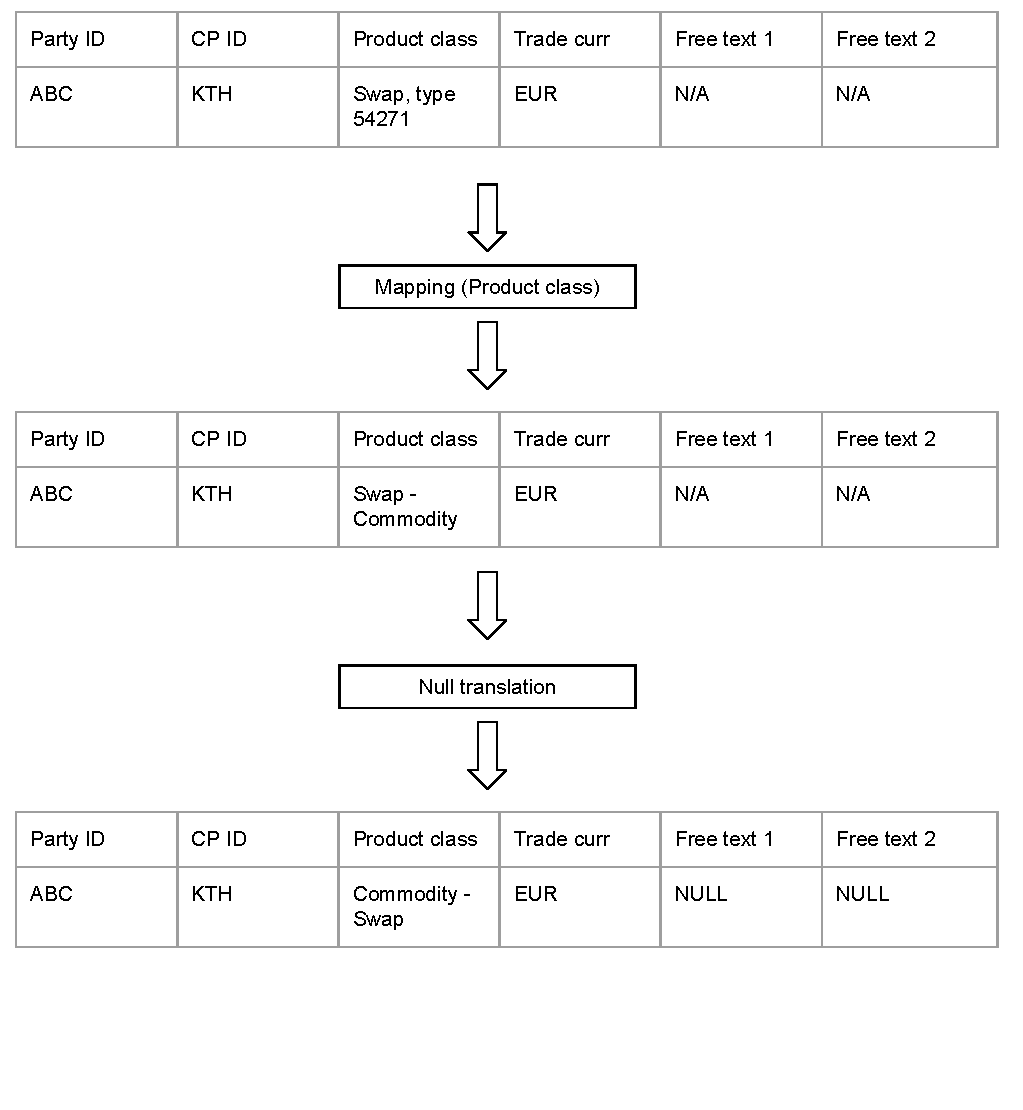
\includegraphics[width=120mm]{figures/filter_diagram.pdf}
  \caption[Filter application example.]{A simplified example of how filter application and dataset transformation work. The mapping filter for the
  product class column is applied, transforming ``Swap, type 54271'' to the standardized ``Swap - Commodity ''. In the file format used for this example,
  ``N/A'' is used to denote the absence of a value, making the null translation filter translate all columns containing ``N/A'' to ``NULL''.}
  \label{fig:filter_diagram}
\end{figure}

\section{Program overview}
The general flow of the original, sequential, dataset processing program is the following:
\\\\
The unprocessed dataset has the rows stored in a Cassandra database, and some metadata and methods stored in a Django object backed by a MySQL database.
The file format corresponding to the dataset is looked up, and all of the filters it contains are added to a pipeline that will process the dataset.
An empty verification result is then created in both Cassandra and MySQL, containing the row data and result metadata with metrics, respectively.
The metrics include processing time, number of trades, timestamp, and similar data. The rows in the dataset are then processed one by one,
applying all filters to each row. As soon as a row has finished processing, it is written to the verification result in Cassandra.
During this process, the row mappings used in the \textit{Mapping} filter are fetched from the MySQL database, resulting in some
I/O waiting time. To mitigate this, the mappings are cached in memory for faster access. After the processing has finished, the result metadata
and metrics are saved in the MySQL database.

A simplified overview of the sequential program can be found in figure \ref{fig:sequential_program_overview}.

\begin{figure}[ht]
  \centering
  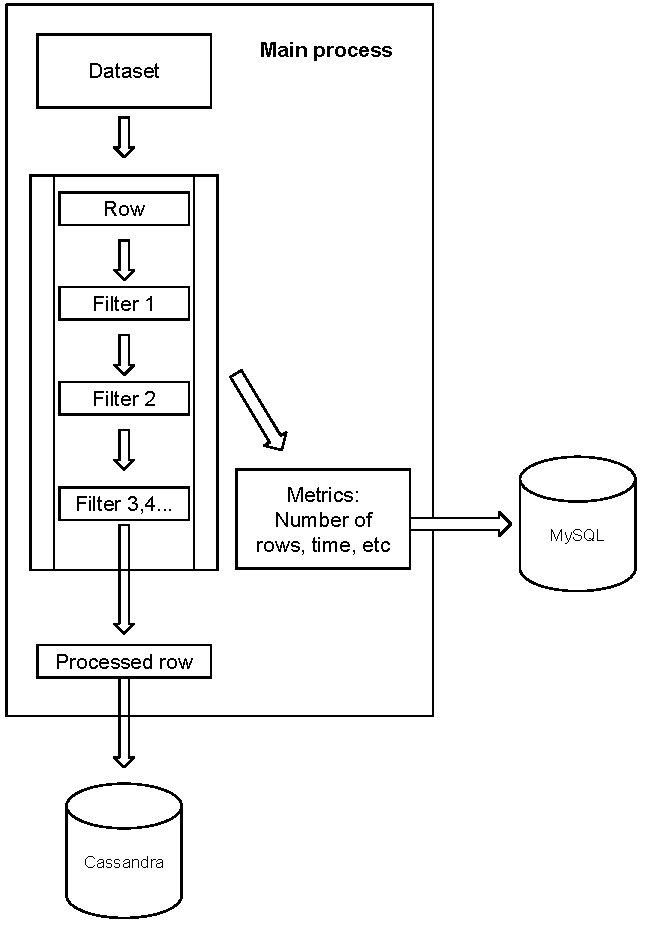
\includegraphics[width=120mm]{figures/program_overview_sequential.pdf}
  \caption[Sequential program overview.]{Sequential program overview.}
  \label{fig:sequential_program_overview}
\end{figure}
